\chapter{Modelldaten\red[Datengrundlage]}
\label{chap.modeldata}
%PreviewVersion
%\red[TODO:\\
%%Verschiedenen Dateitypen nennen?\\
%%Verwendete Programme nennen? Binvox, blender etc.?\\
%Dateistruktur -> Sichern von Daten/Rückkopplung des veränderten Modells hier einfügen?\\
%]

Das Ziel der Anwendung liegt in der Darstellung von Modelldaten durch das \kps{} innerhalb der realen Umgebung. Als Grundlage für die spätere Lokalisation ist es daher erforderlich, ein möglichst originalgetreues Abbild der realen Umgebung zu erstellen. Diese Modellumgebung ermöglicht bei hoher Modellgüte die präzise Positionierung virtueller Objekte in der realen Umgebung.\\
In diesem Kapitel wird die Erstellung einer geeigneten Modellumgebung und der zu visualisierenden Modellobjekte erläutert. Darüber hinaus wird eine Datenstruktur definiert, welche die Repräsentation erstellter Modellszenarien ermöglicht.

%Die zu visualisierenden Modellobjekte werden anhand der virtuellen Umgebungsdaten orientiert und positioniert und können über einen Abgleich in die reale Umgebung übertragen werden. 
%Die Projektion der Modellumgebung selbst innerhalb der realen Umgebung würde lediglich zu Überlagerungen gleicher Strukturen führen und besitzt außerhalb von Validierungen des \kps{s} keine Relevanz.\\

\section{Modellumgebung}
\label{chap.slam}
Für die Verwendung der erstellten Programmstruktur ist es erforderlich, dass die Umgebung in Form eines 3D-Modells abgebildet wird. Als Modellumgebung werden dabei alle statischen Objekte und Strukturen betrachtet, welche eine Repräsentation der realen Umgebung darstellen. Dabei können entweder vorhandene Modelldaten als Basis verwendet oder ein Abbild der Umgebung aus Sensordaten erzeugt werden.\\

Für den Einsatz des \kps{s} mit bestehenden Modelldaten kann das virtuelle Umgebungsmodell direkt aus diesen abgeleitet werden. Insbesondere ist dies der Fall, wenn die Anwendung des \kps{s} in die Planungs- und Bauphase eines Gebäudes integriert werden soll. Eine beispielhafte Modellumgebung ist in \abb{fig.mapMod} dargestellt.\\

\begin{figure}[ht]
	\begin{center}
		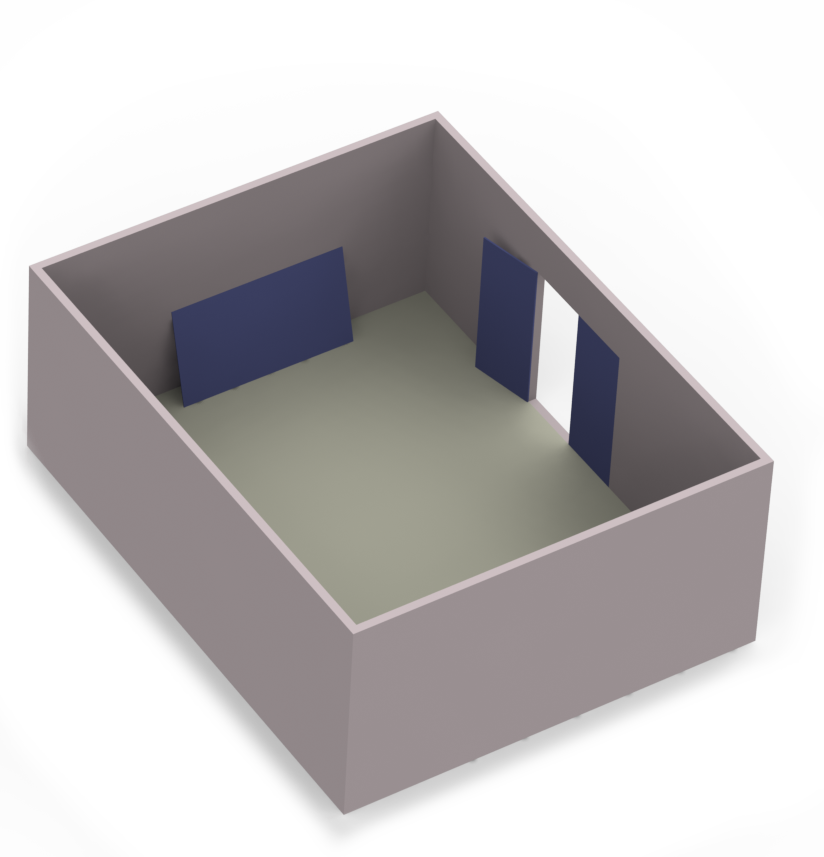
\includegraphics[scale=1.0]{033_cad_02}
		\caption{CAD Modell der Umgebung}
		\label{fig.mapMod}
	\end{center}
	%\vspace*{-8mm}
\end{figure}

Liegen keine Modelldaten vor oder sind diese nicht mehr aktuell, kann ein Abbild der Umgebung auf Basis von Sensordaten erzeugt werden. Diese sogenannte Kartierung von 2D- und 3D-Umgebungen ist in aktuellen Forschungen eng mit der Lokalisation innerhalb dieser Umgebungen verknüpft. Ein verbreitetes Forschungsfeld in diesem Zusammenhang ist das simultane Kartieren und Lokalisieren (SLAM\footnote{\textit{Simultaneous Localization And Mapping} (SLAM) bezeichnet die Erstellung eines Abbildes der Umgebung bei gleichzeitiger Bestimmung der Systempose innerhalb dieser.}) in unbekannten Umgebungen. Dabei existieren verschiedene Algorithmen und Implementierungen zur Lösung der Problemstellungen. Die Kartierung selbst soll in dieser Arbeit nicht näher erläutert werden, für eine detailliertere Darstellung sei deshalb auf \cite{Durrant2006} verwiesen.\\

\nomenclature[a]{SLAM}{Simultaneous Localization and Mapping}

Zur Validierung des Systems wurde die in \abb{fig.mapSLAM} dargestellte Umgebung aufgezeichnet. Dabei wurde eine Implementierung \cite{Rgbdslam} nach Endres \textit{et al.} \cite{Endres2014} verwendet, welche die SLAM Anwendung mittels einer RGB-D Kamera realisiert. Das \kps{} kann somit auch für die Kartierung der Umgebung eingesetzt werden.\\

\begin{figure}[ht]
	\begin{center}
		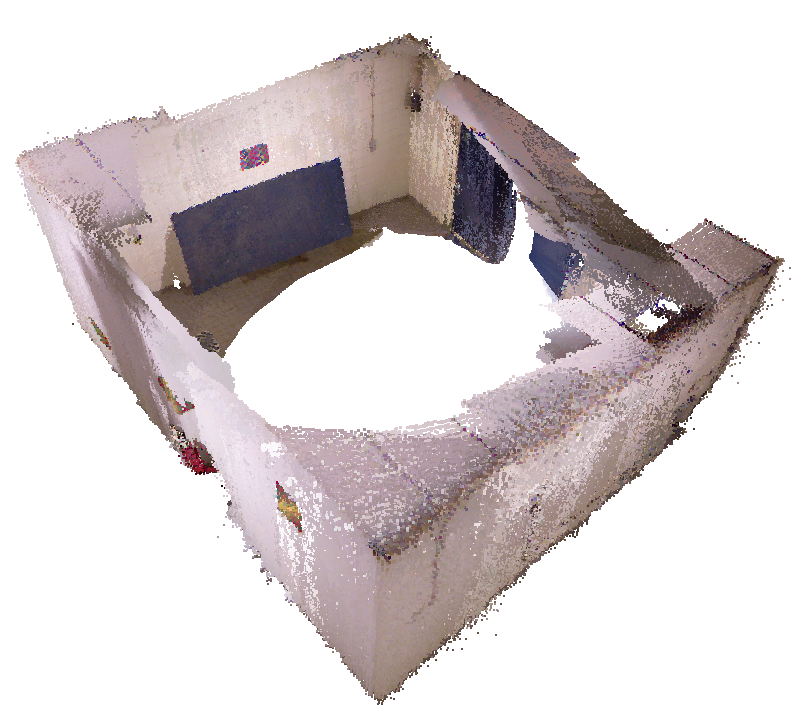
\includegraphics[scale=0.25]{pointcloud_meshlab}
		\caption{Karte RGBDSLAM Subfigures: echter raum (?) - Punktewolke}
		\label{fig.mapSLAM}
	\end{center}
	%\vspace*{-8mm}
\end{figure}

%\red[Boden und Decke nicht modelliert, Limitierungen der Kartenerstellung -> nicht wirklich relevant und führt zu ungenauer Abbildung\\]

Das Ergebnis der Kartierung entspricht einer texturierten Punktwolke. Im Gegensatz zu der Ableitung aus vorhandenen Modelldaten handelt es sich daher nicht um geschlossene Geometrien. Nachteiligen Einfluss können damit die im Vergleich zu Modelldaten geringere Auflösung sowie die Rauscheinflüsse des Kinect-Sensors zeigen. Die Güte eines Modells aus der Kartierung liegt meist unter der Modellgüte bei Ableitung aus vorhandenen 3D-Daten. Um die Fehlereinflüsse zu verringern ist es daher ratsam, die selben Sensoren während der Kartierung und der Lokalisation zu verwenden, da wiederkehrende Sensoreinflüsse so bei beiden Verfahren auftreten.\\

Die erstellte Modellumgebung dient als Basis der späteren Lokalisation und kann zur Visualisierung der Umgebung innerhalb der grafischen Benutzeroberfläche verwendet werden. Die Projektion der Modellumgebung hingegen besitzt außerhalb von Validierungen des \kps{s} keine Relevanz, da sie innerhalb der realen Umgebung lediglich zu Überlagerungen gleicher Strukturen führen würde.\\

\section{Modellobjekte}
Die Projektion visueller Zusatzinformationen basiert auf zu Grunde liegenden virtuellen Modelldaten. Als Modellobjekte werden daher alle Strukturen und Objekte bezeichnet, welche keine Elemente der realen Umgebung abbilden. Zur Modellierung der Objekte können ebenfalls die bei der Erstellung der Modellumgebung eingesetzten Verfahren verwendet werden. Anstelle von Algortihmen zur Kartierung der Umgebung existieren dabei jedoch spezielle Verfahren zur Erfassung dreidimensionaler Objekte, wie beispielsweise von Xu \textit{et al.} \cite{Xu2012} beschrieben.\\

Anders als die Modellumgebung müssen die Modellobjekte nicht als reale Objekte vorhanden sein, weshalb die Modellgüte auch keine Auswirkungen auf die Lokalisations- oder Projektionsgenauigkeit hat. Es können somit beliebige Objekte modelliert werden um diese später in der realen Umgebung zu visualisieren.  Für die Visualisierung ist jedoch eine ausreichende Auflösung der Modellstrukturen und -texturen anzustreben. \abb{fig.modobj} zeigt ein beispielhaftes Modellobjekt und die Integration von Objekten in die Modellumgebung.\\
Die zu visualisierenden Modellobjekte werden anhand der virtuellen Umgebungsdaten orientiert und positioniert und können damit über die im Rahmen der Lokalisation durchgeführte Bestimmung der Systempose in die reale Umgebung projiziert werden.\\

\begin{figure}[ht]
	\begin{center}
	\subfigure[Modellobjekt Steckdose]{
		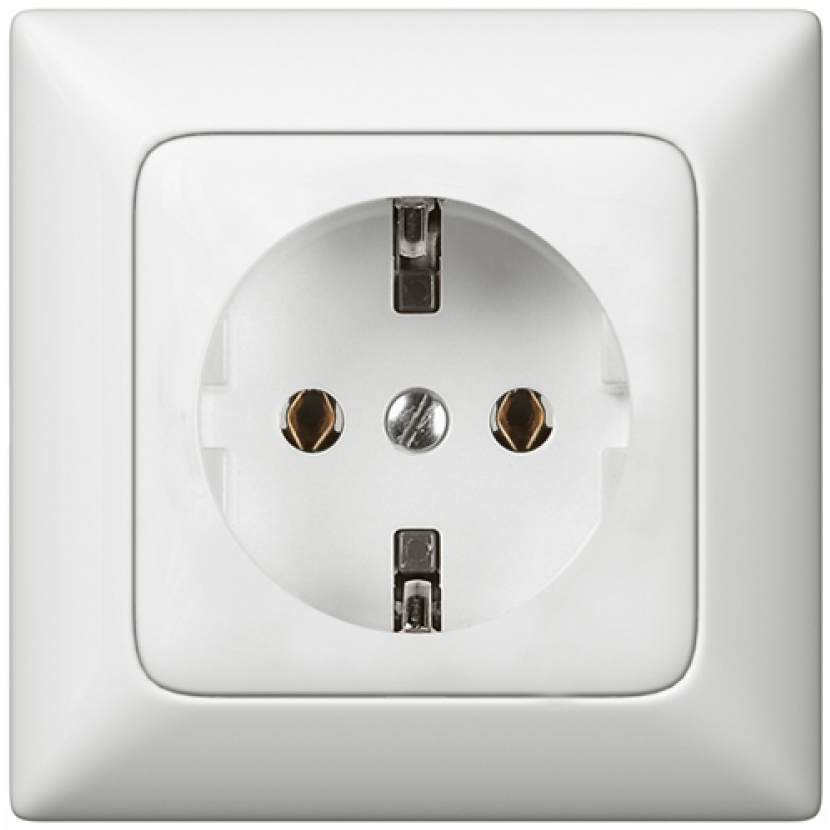
\includegraphics[scale=0.1]{steckdose}
	}
	\hspace{3mm}
%	\subfigure[Modellobjekt elektrische Leitung]{
%			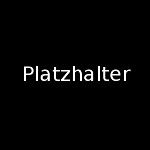
\includegraphics[scale=1.0]{spacer}
%	}
%	\hspace{3mm}
	\subfigure[Modellobjekte in Modellumgebung]{
		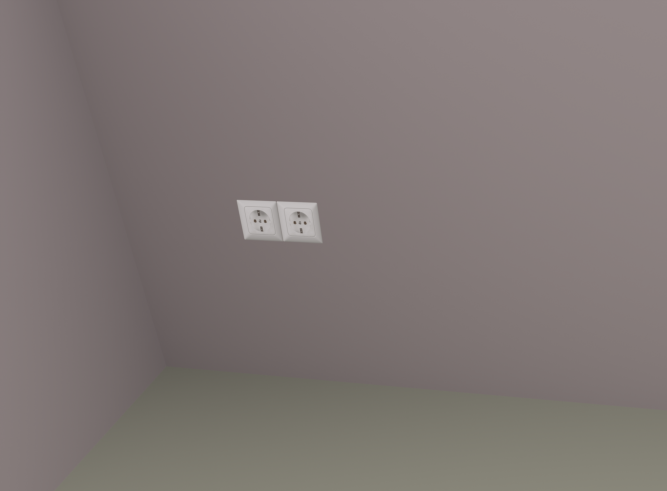
\includegraphics[scale=0.5]{model_obj_cad}
	}
	\caption{Modellobjekte, Subfigures (insgesamt 4, jeweils allein und in Umgebung| Reichen 3? 2xModell + zusammen in Umgebung?): Steckdosen - Leitungen}
	\label{fig.modobj}
	\end{center}
	%\vspace*{-8mm}
\end{figure}

%\red[Modellobjekte ruhig in CAD Umgebung einfügen!\\Vielleicht das Bild von später nehmen?\\]

\section{Datenstruktur}
Um die Szene, bestehend aus der Modellumgebung und allen integrierten Modellobjekten, später wieder in den virtuellen Planungsablauf integrieren zu können wird eine Dateistruktur definiert, welche die Konfiguration der Modellszene repräsentiert. Alle Modellelement werden dazu mit ihrer aktuellen Pose, Textur und geometrischen Repräsentation erfasst, so dass eine Wiederherstellung jederzeit möglich ist. Ein Beispiel, welches den Aufbau der Datenstruktur beschreibt findet sich in \anhang{app.datastructure}\\